% =====================================================================
%  Plan de Investigacion -- UNTREF, Ingenieria de Sonido
%  Compilar:  lualatex main.tex   (dos veces, por las referencias cruzadas)
%  El formato vive entero en untref-plan.cls -- no hace falta tocarlo.
% =====================================================================
\documentclass{untref-plan}

% ------------------------------------------------- datos de la portada
\title{Título del Plan}
\subtitulo{Subtítulo del Plan (si lo tuviera)}
\author{Nombre y apellido (DNI número)}
\tutor{Nombre y apellido}
\cotutor{Nombre y apellido (si lo tuviera))}   % borrar esta línea si no hay cotutor
\defensa{Fecha de defensa: mes y año | Locación (ej.\ Sáenz Peña), Argentina}
\tituloinvestigacion{Título de la Investigación}
\investigador{Nombre del Investigador}

\begin{document}
\maketitle

% =====================================================================
\section{Fundamentación e Introducción.}

En la fundamentación debe desarrollarse la pregunta que lleva a la investigación y su justificación. Es habitual incorporar aquí una visión rápida sobre el estado del tema de estudio (la que se profundizará en el Estado del Arte). Lo importante es dejar claro que la investigación que se pretende desarrollar, va a llenar algún punto vacío en la ciencia o en la tecnología. El desarrollo mínimo de este punto es una carilla.

La introducción debe finalizar con un resumen de cada una de las partes que forman la investigación, es decir una rápida descripción de lo que va a desarrollarse en cada uno de los títulos o capítulos del documento.

% =====================================================================
\section{Objetivos General y específicos.}

El objetivo general debe ser expresado en un solo párrafo, de ser posible en una sola oración, y debe reflejar la pregunta que dio origen a la investigación. Los objetivos específicos deben redactarse uno por uno, recordando que el objetivo general se alcanza cumpliendo con todos los objetivos específicos.

Los objetivos específicos se desarrollan como un punteo de las acciones de la investigación que van a realizarse. El análisis de la bibliografía no es un objetivo específico. Podría serlo en caso que se pretenda repetir alguna experiencia de la bibliografía o del estado del arte para verificar alguna cosa. Los objetivos específicos pueden plantearse como sigue:

\begin{itemize}
  \item Lorem ipsum dolor sit amet consectetur, adipiscing elit orci.
  \item Id primis lacinia diam massa, torquent pulvinar metus.
  \item Odio turpis mi fermentum rhoncus, mus fames.
  \item Interdum parturient lacinia tellus penatibus ad, tempor justo morbi.
  \item Felis praesent vitae neque porttitor vel, vulputate porta tristique mus.
\end{itemize}

% =====================================================================
\section{Marco Teórico y Estado del Arte.}

En el Marco Teórico debemos incorporar la bibliografía, artículos de revistas, ponencias de congresos, links de Internet o todo aquello que haya contribuido a formar el cuerpo del saber sobre el que va a basarse la investigación, incorporando los procesos y ecuaciones necesarios. En el Estado del arte se hará una revisión de las últimas investigaciones sobre el tema que pretendemos investigar, realizando una breve descripción de los puntos de interés de cada una. \textbf{No pueden indicarse menos de 12 referencias} para este plan de investigación.

% =====================================================================
\section{Diseño de la Investigación.}

El diseño de investigación implica desarrollar las previsiones generales del plan para el experimento, definiendo el tipo de investigación a realizar, su alcance, etc. Dado que en este ejercicio se trata de evaluar subjetivamente alguna variable, debe explicarse en términos amplios el plan a desarrollar, el que se pormenorizará en los puntos siguientes. Es importante explicar todo el diseño para que se tenga una visión completa, sin redundar en las explicaciones que van a realizarse en los puntos que siguen. De este modo, el lector o evaluador del proyecto, tienen una primera impresión de la totalidad.

\subsection{Diseño prueba objetiva: Definición de Variables. Muestra.}

Está claro que si la investigación no tiene una parte subjetiva, el título de este ítem será: Diseño de la Investigación, variables y muestra.

En esta parte deben definirse las variables que serán medidas, y cuáles son las que se estima llevar a la evaluación subjetiva. Debe incluirse un diagrama de los equipos a emplear en las mediciones y un diseño preciso de cómo se llevarán a cabo.

Las ecuaciones y expresiones matemáticas deben estar centradas y numeradas en secuencia, con el número de la ecuación a la derecha y entre paréntesis, utilizando numeración arábiga. En ecuaciones de varias líneas, la numeración debe ser ubicada en la última línea. Las fórmulas y el texto deben ser separados por una línea. Las ecuaciones deben ser hechas en la misma fuente del texto, con los índices 3 puntos abajo. Deben usarse símbolos convencionales y unidades SI. Las ecuaciones deben ser citadas en el texto (``Ecuación~(\ref{eq:ejemplo})'', etc.):

\begin{equation}\label{eq:ejemplo}
  R' = L_1 - L_2 + 10\log\!\left(\frac{S}{A}\right) \quad \mathrm{dB}
\end{equation}

\begin{figure}[h]
  \centering
  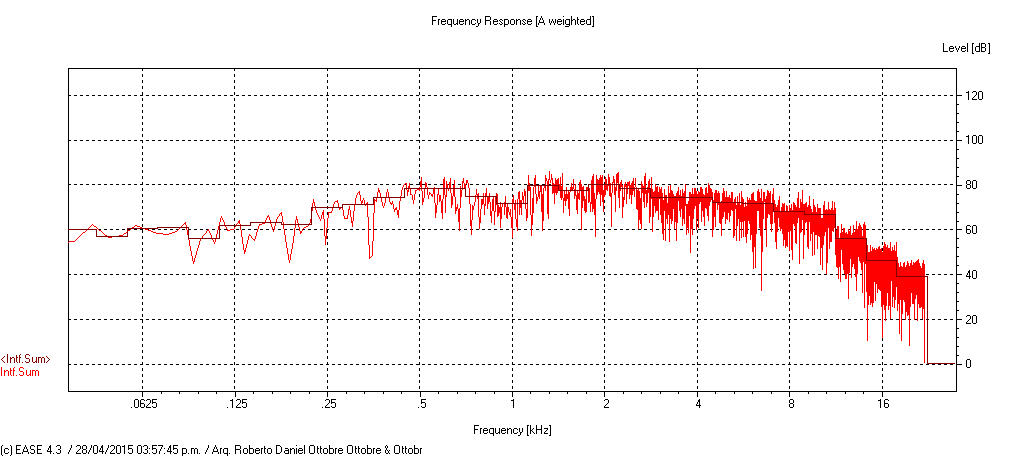
\includegraphics[width=15.39cm,height=6.80cm]{figuras/ejemplo-figura.png}
  \caption{Figuras centradas con títulos al pie.}
  \label{fig:ejemplo}
\end{figure}

\subsection{Diseño prueba subjetiva: Encuesta y Muestra. (si existiera una prueba subjetiva)}

En primer lugar debe definirse si se recurrirá a una muestra probabilística o no probabilística, la cantidad de sujetos que se encuestarán, y la justificación de ese decisión. Aquí debe desarrollarse también de modo completo el cuestionario y el desarrollo de la encuesta, es decir definir las preguntas, las muestras que se presentarán a los encuestados, las series de pruebas, duración, etc. Debe incluso definirse con exactitud el recorrido que hará cada encuestado, el lugar, las características del equipamiento a emplear, etc.

\section{Validación de las pruebas.}

Las pruebas se validarán siguiendo los criterios estadísticos que permiten determinar la existencia o no de errores en alguna o algunas encuestas y considerar si son incluidas o no en el conjunto de respuestas. Como las pruebas no se realizarán todavía, deben plantearse los métodos elegidos y explicarlos.

\section{Análisis de los resultados: Aplicaciones estadísticas.}

Aquí se aplicarán los métodos estadísticos que nos permitan concluir los resultados y proyectar diferentes facetas de los datos obtenidos. Como las pruebas no se realizarán todavía, deben plantearse los métodos elegidos y explicarlos.

\begin{figure}[h]
  \centering
  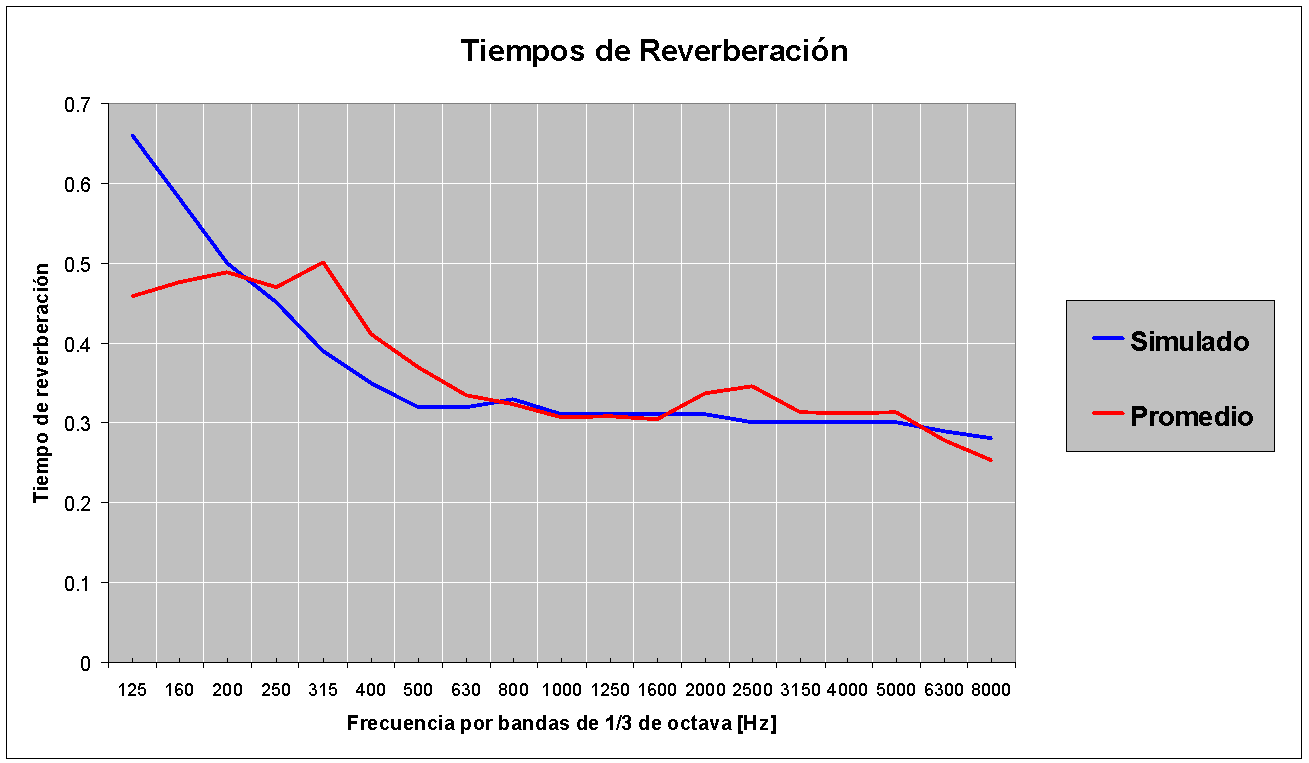
\includegraphics[width=11.09cm,height=6.46cm]{figuras/figura-2.png}
  \caption*{Figure 2. Comparison of the reverberation times between the spatial-average and the simulation for Hall 4.}
\end{figure}

\begin{figure}[h]
  \centering
  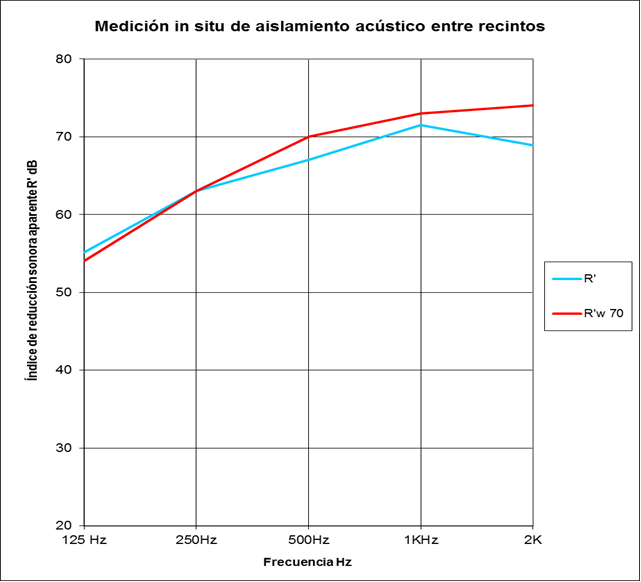
\includegraphics[width=10.76cm,height=9.73cm]{figuras/figura-3.png}
  \caption*{Figure 3. Sound insulation index according to IRAM 4063-4.}
\end{figure}

% =====================================================================
\section{Conclusiones.}

En las conclusiones del Plan de Investigación, debe plantearse cómo será la exposición de los resultados y qué es lo que se espera obtener en resumen de las pruebas que se realicen.

% =====================================================================
\section{Líneas futuras de investigación.}

Las líneas futuras de investigación dentro del plan, suponen expresar qué posibles cuestiones que se encontrarán se dejarán para ser profundizadas más adelante por otras investigaciones.

% =====================================================================
\section{Cronograma.}

El siguiente diagrama de Gantt enuncia el cronograma de actividades y tareas previstas al momento de la realización de la investigación.

\bigskip
% \gX = semana marcada (celda con relleno gris, igual que el .docx).
% La primera columna va vacia en el modelo: poner ahi el nombre de cada tarea.
\begin{gantt}
 &\gX&   &   &   &   &   &   &   &   &   &   &   & & & & \tabularnewline\hline
 &\gX&   &   &   &   &   &   &   &   &   &   &   & & & & \tabularnewline\hline
 &\gX&   &   &   &   &   &   &   &   &   &   &   & & & & \tabularnewline\hline
 &\gX&\gX&   &   &   &   &   &   &   &   &   &   & & & & \tabularnewline\hline
 &   &   &\gX&   &   &   &   &   &   &   &   &   & & & & \tabularnewline\hline
 &   &   &   &\gX&\gX&\gX&   &   &   &   &   &   & & & & \tabularnewline\hline
 &   &   &   &   &   &\gX&\gX&\gX&   &   &   &   & & & & \tabularnewline\hline
 &   &   &   &   &   &   &   &   &\gX&\gX&\gX&\gX&\gX&\gX&\gX&\gX \tabularnewline\hline
\end{gantt}
\bigskip

% =====================================================================
% Referencias en APA (https://untref.edu.ar/raesta/normas-apa.php)
% Sangría francesa de 0.75 cm, justificado, 12 pt -- una entrada por párrafo.
\begin{referencias}

Beranek, L. (2004). Concert halls and opera houses: Music, Acoustics, and Architecture (2nd ed.). Springer.

Busch-Vishniac, I. J., West, J. E., Barnhill, C., Hunter, T., Orellana, D., \& Chivukula, R. (2005). Noise levels in Johns Hopkins Hospital. The Journal of the Acoustical Society of America, 118(6), 3629–3645. https://doi.org/10.1121/1.2118327

Call, R. B. (2007). Sound practices: Noise control in the healthcare environment. AAH Academy Journal, 10, 9 pages.

https://www.brikbase.org/content/sound-practices-noise-control-healthcare-environment

Gardner, W. G. (2002). Reverberation algorithms. In M. Kahrs (Ed.), Applications of digital signal processing to audio and acoustics (Vol. 437). Springer.

International Organization for Standardization. (2017). Acoustics – description, measurement and assessment of environmental noise — part 2: Determination of sound pressure levels (Standard No. ISO 1996-2:2017).

Kracht, J. M., Busch-Vishniac, I. J., \& West, J. E. (2007). Noise in the Operating Rooms of Johns Hopkins Hospital. The Journal of the Acoustical Society of America, 121(5), 2673–2680. https://doi.org/10.1121/1.2714921

Lawson, N., Thompson, K., Saunders, G., Saiz, J., Richardson, J., Brown, D., Ince, N., Caldwell, M., \& Pope, D. (2010). Sound intensity and noise evaluation in a Critical Care Unit. American Journal of Critical Care, 19(6). https://doi.org/10.4037/ajcc2010180

MacLeod, M., Dunn, J., Busch-Vishniac, I. J., West, J. E., \& Reedy, A. (2007). Quieting Weinberg 5C: A case study in hospital noise control. The Journal of the Acoustical Society of America, 121(6), 3501–3508. https://doi.org/10.1121/1.2723655

Mazer, S. E. (2012). Creating a culture of safety: Reducing hospital noise. Biomedical Instrumentation \& Technology, 46(5), 350–355. https://doi.org/10.2345/0899-8205-46.5.350

Orellana, D., Busch-Vishniac, I. J., \& West, J. E. (2006). Noise in the adult emergency department of Johns Hopkins Hospital. The Journal of the Acoustical Society of America, 119(5\_Supplement), 3385–3385. https://doi.org/10.1121/1.4786628

Richardson, A., Thompson, A., Coghill, E., Chambers, I., \& Turnock, C. (2009). Development and implementation of a noise reduction intervention programme: A pre- and postaudit of three hospital wards. Journal of Clinical Nursing, 18(23), 3316–3324. https://doi.org/10.1111/j.1365-2702.2009.02897.x

Ryherd, E. E., Waye, K. P., \& Ljungkvist, L. (2008). Characterizing noise and perceived work environment in a neurological intensive care unit. The Journal of the Acoustical Society of America, 123(2), 747–756. https://doi.org/10.1121/1.2822661

Sanz Vila, C. (2012). Técnicas para el estudio acústico en vehículos (Tesis de Master). Universidad Politécnica de Valencia, Spain.

Taylor, F. B. (1958). Noise control in a Research Hospital. Noise Control, 4(5), 9–62. https://doi.org/10.1121/1.2369339

Tsiou, C., Efthymiatos, G., \& Katostaras, T. (2008). Noise in the Operating Rooms of Greek hospitals. The Journal of the Acoustical Society of America, 123(2), 757–765. https://doi.org/10.1121/1.2821972

Text-to-Speech - IBM Cloud. (2021). Retrieved October 6, 2021, from https://cloud.ibm.com/ catalog/services/text-to-speech

West, J. E. (2008). Noise in hospitals: Effects and cures. Annual Harold W. Gegenheimer Lecture Series on Innovation. http://hdl.handle.net/1853/26201

https://untref.edu.ar/raesta/normas-apa.php

\end{referencias}

\end{document}
